% tikzpic.tex
\documentclass[crop]{standalone}% 'crop' is the default for v1.0, before it was 'preview'
\usepackage{testpackage}
\setromanfont{Fira Sans}
\setmainfont{Fira Sans}
\everymath\expandafter{\the\everymath\rm}
\everydisplay\expandafter{\the\everydisplay\rm}
%\usetikzlibrary{...}% tikz package already loaded by 'tikz' option
\usepackage{tikz,pgfplots}
\usepackage{array}




\begin{document}
	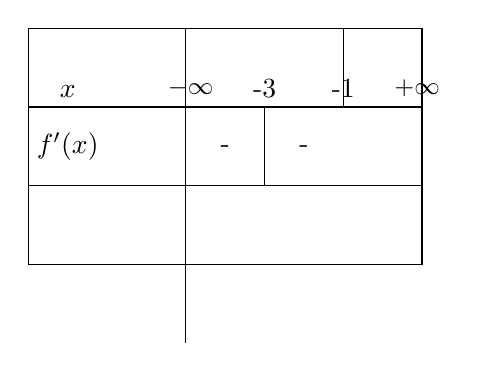
\begin{tikzpicture}
	\draw (0,4) rectangle (5,6);
	\draw (0,3) rectangle (5,4);
	\draw (2,2)--(2,6);
	\draw(0,4)--(5,4);
	\draw(0,5)--(5,5);
	\draw(3,4)--(3,5) node[above]{-3};
	\draw(4,6)--(4,5)node[above]{-1};
	\node[above right,xshift=-10] at (2,5){\small$-\infty$};
	\node[above left,xshift=10] at (5,5){\small$+\infty$};
	\node at (0.5,4.5){$f'(x)$};\node at (2.5,4.5){-};\node at (3.5,4.5){-};
	\node [above]at (0.5,5){$x$};
	\end{tikzpicture}
\end{document}